\section{ИЗМЕРЕНИЕ ВРЕМЕНИ И РЕЗУЛЬТАТЫ}
Время работы программы измерялась с помощью функции \texttt{clock()}. Для измерения времени решения задачи в последовательном режиме была написана функция \texttt{taskCPU}, код которой представлен в Листинге \ref{listing:taskCPU}.
\begin{lstlisting}[style=CStyle, label={listing:taskCPU}, caption={Функция, измеряющая время работы последовательного решения задачи.}]
float taskCPU(int n){
	// Arrays declaration
	float *hostA, *hostB;
	clock_t t1, t2;
	// CPU variant
	t1 = clock();
	// Arrays allocation
	hostA = (float*)malloc(n*sizeof(float));
	hostB = (float*)malloc(n*sizeof(float));
	// Arrays initialization
	for (int i=0; i<n; i++){
		hostA[i] = (float)rand()/(float)(RAND_MAX);
		hostB[i] = (float)rand()/(float)(RAND_MAX);
	}
	// Print array
	if (isPrint) printf("A\t");
	if (isPrint) printArray(hostA, n);
	if (isPrint) printf("B\t");
	if (isPrint) printArray(hostB, n);
	// Sorting
	bubbleSortCPU(hostA, n);
	bubbleSortCPU(hostB, n);
	// Print arrays
	if (isPrint) printf("sorted A\t");
	if (isPrint) printArray(hostA, n);
	if (isPrint) printf("sorted B\t");
	if (isPrint) printArray(hostB, n);
	// Dot product
	float dot_prod = dotProdCPU(hostA, hostB, n);
	if (isPrint) printf("dot_prods\t%f\n", dot_prod);
	t2 = clock();
	// Release memory
	free(hostA);
	free(hostB);
	return (float)(t2-t1)/CLOCKS_PER_SEC;
}
\end{lstlisting}

Аналогично, для измерения времени решения задачи в оптимизированном с использованием CUDA режиме была написана функция \texttt{taskCUDA}, код которой представлен в Листинге \ref{listing:taskCUDA}.
\begin{lstlisting}[style=CStyle, label={listing:taskCUDA}, caption={Функция, измеряющая время работы оптимизированного с использованием CUDA решения задачи.}]
float taskCUDA(int n){
	// Arrays declaration
	float *hostA, *hostB;
	clock_t t1, t2;
	// CPU variant
	if (isPrint) printf("CUDA is not used\n");
	t1 = clock();
	// Arrays allocation
	hostA = (float*)malloc(n*sizeof(float));
	hostB = (float*)malloc(n*sizeof(float));
	// Arrays initialization
	for (int i=0; i<n; i++){
		hostA[i] = (float)rand()/(float)(RAND_MAX);
		hostB[i] = (float)rand()/(float)(RAND_MAX);
	}
	// Print array
	if (isPrint) printf("A\t");
	if (isPrint) printArray(hostA, n);
	if (isPrint) printf("B\t");
	if (isPrint) printArray(hostB, n);
	// Sorting
	bubbleSortCUDA(hostA, n);
	bubbleSortCUDA(hostB, n);
	// Print arrays
	if (isPrint) printf("sorted A\t");
	if (isPrint) printArray(hostA, n);
	if (isPrint) printf("sorted B\t");
	if (isPrint) printArray(hostB, n);
	// Dot product
	float dot_prod = dotProdCUDA(hostA, hostB, n);
	if (isPrint) printf("dot_prods\t%f\n", dot_prod);
	t2 = clock();
	// Release memory
	free(hostA);
	free(hostB);
	return (float)(t2-t1)/CLOCKS_PER_SEC;
}
\end{lstlisting}

В ходе тестирования было выявлено, что свободные параметры CUDA-версии алгоритма \texttt{blockSizeBubbleSort} и \texttt{blockSizeDotProd} слабо влияют на время работы программы, поэтому тут и далее они полагаются равными 1024. Сравнение времени работы программы в двух режимах приводится на Рис. \ref{fig:time} и в Таблицах \ref{tab:cpu_time} и \ref{tab:cuda_time}.
\begin{figure}
    \centering
    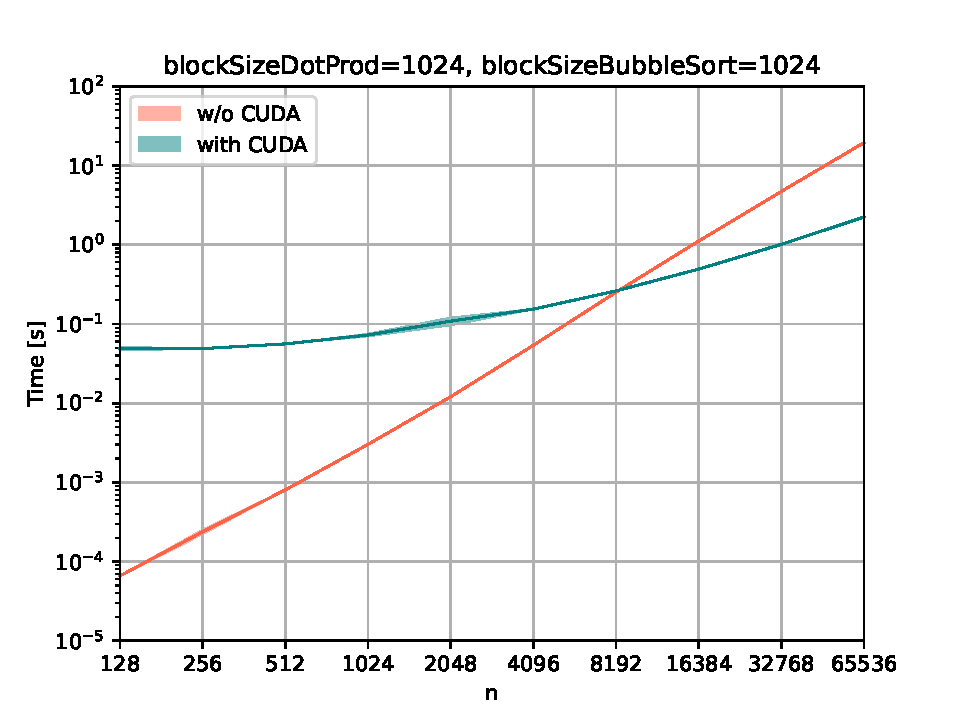
\includegraphics{fig/time.pdf}
    \caption{Сравнение времени работы реализаций алгоритма решения задачи в двух исполнениях: с использованием  CUDA (with CUDA) и без CUDA (w/o CUDA). Закрашенные области вокруг кривых соответствуют среднекравдратичному отклонению (они могут быть плохо заметны из-за своей малости).}
    \label{fig:time}
\end{figure}
Видно, что при малых n быстрее оказывается последовательная версия, но при n > 8192 более эффективной оказывается алгоритм, оптимизированный с помощью CUDA.